\documentclass[landscape,a4paper,12pt,french, twocolumn]{article}

\usepackage{../../../Style}

\renewcommand\tabularxcolumn[1]{m{#1}}

% Début du document
%%%%%%%%%%%%%%%%%%%
\begin{document}

\title{\vspace{-1cm} Fonctions: Généralités \vspace{-1cm} }
\author{}
\date{}
\maketitle

%\begin{FlushLeft}

\section{Définitions, notations}

\begin{defin}
Soit $D \subset \R$. On appelle fonction $f$ sur l'ensemble $D$ le processus qui à tout nombre $x \in D$ associe un \textbf{unique} réel noté $f(x)$. On note $\fonction f D {\R} x {f(x)}$.
\begin{center}
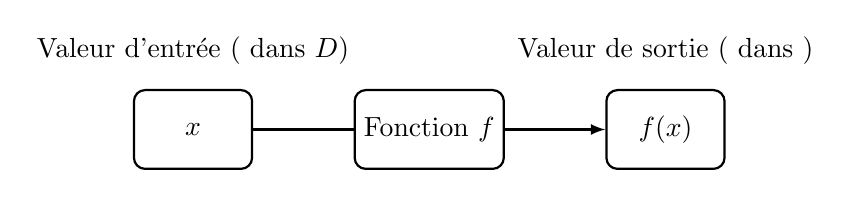
\begin{tikzpicture}[scale=1]
\node[draw,rectangle,thick, minimum height=10mm, minimum width=15mm, rounded corners] (x) at (-3,0) {$x$};
\node[yshift=10mm] at (x) {Valeur d'entrée ( dans $D$)};
\node[draw,rectangle,thick, minimum height=10mm, minimum width=15mm, rounded corners] (f) at (0,0) {Fonction $f$};
\node[draw,rectangle,thick, minimum height=10mm, minimum width=15mm, rounded corners] (fx) at (3,0) {$f(x)$};
\node[yshift=10mm] at (fx) {Valeur de sortie ( dans $\R$)};
\draw[-,>=latex,thick] (x) to (f);
\draw[->,>=latex,thick] (f) to (fx);
\end{tikzpicture}
\end{center}

On dit alors que:
\begin{itemize}
\item $f(x)$ est l'image de $x$
\item $x$ est un antécédent de $f(x)$
\item $D$ est l'ensemble ( ou domaine ) de définition de $f$
\end{itemize}

\end{defin}

\begin{ex}
On définit la fonction $\fonction f {\R} {\R} x {x^2-x}$.
\begin{itemize}
\item L'ensemble de définition de $f$ est $\R$.
\item L'image de $2$ par la fonction $f$ est $2$: $f(2)=2^2-2=2$.
\item $2$ est un antécédent de $2$ par la fonction $f$. $-1$ en est aussi un car $f(-1)=(-1)^2+1=2$.
\end{itemize}
\end{ex}

\begin{rmq}
Chaque nombre dans $D$ possède une unique image, mais plusieurs antécédents d'un même nombre peuvent exister.
\end{rmq}

\section{Représentation graphique d'une fonction}

\begin{defin}
Dans un repère du plan, l'ensemble des points $(x,f(x))$ pour $x \in D$ constitue la courbe de $f$. L'équation de la courbe de $f$ est $y=f(x)$ pour $x \in D$.
\end{defin}

Dans la pratique, il faut placer plusieurs points pour tracer la courbe d'une fonction le plus précisément possible. On peut s'aider d'une table de valeurs.

\begin{center}
\begin{tabularx}{0.95\linewidth}{ 
  | >{\centering\arraybackslash}c 
  | >{\centering\arraybackslash}X
  | >{\centering\arraybackslash}X
  | >{\centering\arraybackslash}X
  | >{\centering\arraybackslash}X
  | >{\centering\arraybackslash}X
  | >{\centering\arraybackslash}X
  | >{\centering\arraybackslash}X
  | >{\centering\arraybackslash}X
  | >{\centering\arraybackslash}X| } \hline
$x$ & $-1.5$ & $-1$ & $-0.5$ & $0$ & $0.5$ & $1$ & $1.5$ & $2$ & $2.5$ \\ \hline
$f(x)$ & & & & & & & & &\rule[-7pt]{0pt}{30pt} \\ \hline
\end{tabularx}
\end{center}

\begin{center}
\begin{tikzpicture}[scale=\echellepgf]
\begin{axis}[
axis x line=bottom,
axis y line = left,
axis lines=middle,
width=0.9*\echellepgfinv*\linewidth,
height=\pgfkeysvalueof{/pgfplots/width}*((\pgfkeysvalueof{/pgfplots/ymax})+((-1)*(\pgfkeysvalueof{/pgfplots/ymin})))/((\pgfkeysvalueof{/pgfplots/xmax})+((-1)*(\pgfkeysvalueof{/pgfplots/xmin})))+0.05pt,
scale only axis,
xmin=-3.5, xmax=3.5,
ymin=-1, ymax=4,
xlabel={$x$},
ylabel={$y$},
minor x tick num=1,
minor y tick num=1,
xtick distance=1,
ytick distance=1,
grid=both,
grid style=dashed,
axis equal,
legend pos=north west,
]
\addplot[samples=101,smooth,ultra thick,domain=(-3:3),mark=none]{x^2-x} node [pos=0.85,right] {$\mathscr C_f$};
%\addplot[samples=13,smooth,ultra thick,domain=(-3:3),mark=*,color=red, only marks]{x^2-x};
\addlegendentry{$f(x)=x^2-x$};
\pgfplotsinvokeforeach{-1.5,-1,...,2.5}{ \node[circle, minimum size=2pt,fill,color=red,inner sep=2pt] at (axis cs:#1,#1*#1-#1) {};}

\addplot +[mark=none,color=blue,style=dashed,very thick] coordinates {(2.2, 0) (2.2, 2.2^2-2.2)} node [pos=0,below] {$x$};
\addplot +[mark=none,color=blue,style=dashed,very thick] coordinates {(2.2, 2.2^2-2.2) (0, 2.2^2-2.2)} node [pos=1,left] {$f(x)$};
\node[circle, minimum size=1pt,fill,color=blue,inner sep=2pt] at (axis cs:2.2,2.2^2-2.2) {};
%\addplot +[mark=none,color=red,style=dashed,very thick] coordinates {(-1, 0) (-1, 2)};
%\addplot +[mark=none,color=red,style=dashed,very thick] coordinates {(-1, 2) (0, 2)};
%\node[label={0:{$(0,1)$}},rectangle,fill,inner sep=2pt] at (axis cs:0,1) {};
%\node[label={[label distance=2pt]-90:{$(0,1)$}},rectangle,fill,inner sep=0pt, minimum height=0pt, minimum width=4pt] at (axis cs:1,1) {};
\end{axis}
\end{tikzpicture}
\end{center}

Les points $(-1;2)$ et $(1;0)$ appartiennent à la courbe de $f$, mais pas le point $(0;1)$.

\newpage
\section{Résolution graphique d'équations et d'inéquations}

\renewcommand\tabularxcolumn[1]{p{#1}}

\subsection{Equations}

\vspace{-5mm}
\begin{center}
\resizebox{\linewidth}{!}{
\begin{tabularx}{0.8\textwidth}{|X|X| } \hline
\Centering{$f(x)=k$} & \Centering{$f(x)=g(x)$} \\ \hline
\Centering{
\begin{tikzpicture}[scale=1]
\begin{axis}[
axis x line=bottom,
axis y line = left,
axis lines=middle,
width=1.1*\linewidth,
height=0.8*\linewidth,
xmin=-0.5, xmax=4.5,
ymin=-1, ymax=4,
enlargelimits={abs=0.2},
xlabel={$x$},
ylabel={$y$},
%ytick distance=1,
ticks=none,
grid style=dashed,
%axis equal,
legend pos=north east,
xlabel style={at={(ticklabel* cs:0.95)},below=0.1},
]
\addplot[samples=101,smooth,ultra thick,domain=(-2:5),mark=none]{3.5*e^(-0.4*(x-2)^2)} node [pos=0.75,right] {$\mathscr C_f$};

\addplot +[mark=none,color=blue,style=dashed,very thick] coordinates {(-1,2.8) (5, 2.8)} node [pos=0.18,above right] {$k$};
\node[circle, minimum size=1pt,fill,color=blue,inner sep=2pt] at (axis cs:1.25,2.8) {};
\node[circle, minimum size=1pt,fill,color=blue,inner sep=2pt] at (axis cs:2.75,2.8) {};
\addplot +[mark=none,color=blue,style=dashed,very thick] coordinates {(1.25,0) (1.25, 2.8)} node [pos=0,below] {$x_1$};
\addplot +[mark=none,color=blue,style=dashed,very thick] coordinates {(2.75,0) (2.75, 2.8)} node [pos=0,below] {$x_2$};
%\addplot +[mark=none,color=red,style=dashed,very thick] coordinates {(-1, 0) (-1, 2)};
%\addplot +[mark=none,color=red,style=dashed,very thick] coordinates {(-1, 2) (0, 2)};
%\node[label={0:{$(0,1)$}},rectangle,fill,inner sep=2pt] at (axis cs:0,1) {};
%\node[label={[label distance=2pt]-90:{$(0,1)$}},rectangle,fill,inner sep=0pt, minimum height=0pt, minimum width=4pt] at (axis cs:1,1) {};
\end{axis}
\end{tikzpicture}}
&
\Centering{
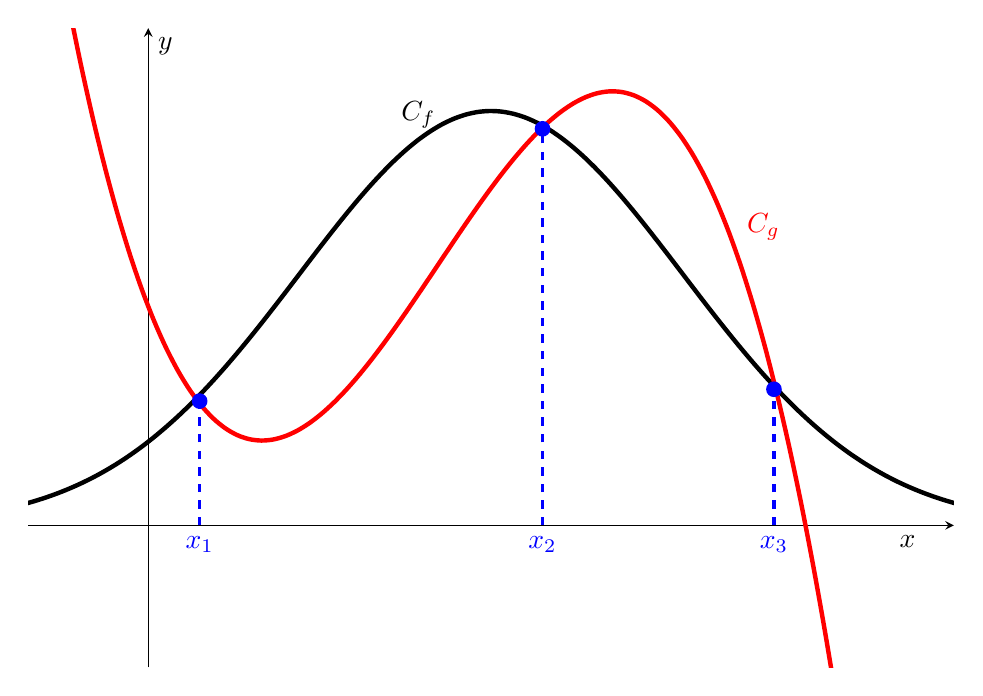
\begin{tikzpicture}[scale=1]
\begin{axis}[
axis x line=bottom,
axis y line = left,
axis lines=middle,
width=1.1*\linewidth,
height=0.8*\linewidth,
xmin=-0.5, xmax=4.5,
ymin=-1, ymax=4,
enlargelimits={abs=0.2},
xlabel={$x$},
ylabel={$y$},
ticks=none,
%ytick distance=1,
%axis equal,
yticklabel=\empty,
xticklabel=\empty,
xlabel style={at={(ticklabel* cs:0.95)},below=0.1},
]
\addplot[samples=101,smooth,ultra thick,domain=(-2:5),mark=none]{3.5*e^(-0.4*(x-2)^2)} node [pos=0.5,above] {$\mathscr C_f$};
\addplot[samples=101,smooth,ultra thick,domain=(-2:5),mark=none,color=red]{-0.69*x^3+3.49*x^2-3.72*x+1.85} node [pos=0.65,above right,color=red] {$\mathscr C_g$};

\addplot +[mark=none,color=blue,style=dashed,very thick] coordinates {(0.3,0) (0.3, 1.05)} node [pos=0,below] {$x_1$} node[pos=1,circle, minimum size=1pt,fill,inner sep=2pt] {};
\addplot +[mark=none,color=blue,style=dashed,very thick] coordinates {(2.3,0) (2.3, 3.35)} node [pos=0,below] {$x_2$} node[pos=1,circle, minimum size=1pt,fill,inner sep=2pt] {};
\addplot +[mark=none,color=blue,style=dashed,very thick] coordinates {(3.65,0) (3.65, 1.15)} node [pos=0,below] {$x_3$} node[pos=1,circle, minimum size=1pt,fill,inner sep=2pt] {};
%\addplot +[mark=none,color=red,style=dashed,very thick] coordinates {(-1, 0) (-1, 2)};
%\addplot +[mark=none,color=red,style=dashed,very thick] coordinates {(-1, 2) (0, 2)};
%\node[label={0:{$(0,1)$}},rectangle,fill,inner sep=2pt] at (axis cs:0,1) {};
%\node[label={[label distance=2pt]-90:{$(0,1)$}},rectangle,fill,inner sep=0pt, minimum height=0pt, minimum width=4pt] at (axis cs:1,1) {};
\end{axis}
\end{tikzpicture}}
\\ \hline
Résoudre l'équation $f(x)=k$ signifie trouver les antécédents de $k$ par la fonction $f$.

Cela revient donc à chercher l'abscisse des points d'intersection de la courbe avec la droite d'équation $y=k$.

Ici, l'ensemble des solution de l'équation est:$$S=\{x_1,x_2 \}$$ \vspace{-5mm}
&
Résoudre l'équation $f(x)=k$ signifie trouver les nombres qui ont la même image par $f$ et $g$.

Cela revient donc à chercher l'abscisse des points d'intersection des deux courbes $\mathscr C_f$ et $\mathscr C_g$.

Ici, l'ensemble des solution de l'équation est:$$S=\{x_1,x_2,x_3 \}$$ \vspace{-5mm} \\ \hline
\end{tabularx}}
\end{center}

\subsection{Inéquations}

\vspace{-5mm}
\begin{center}
\resizebox{\linewidth}{!}{
\begin{tabularx}{0.8\textwidth}{ |X|X|X| } \hline
\Centering{$f(x) \geq k$} & \Centering{$f(x)<k$} & \Centering{$f(x)>g(x)$} \\ \hline
\multicolumn{2}{|c|}{
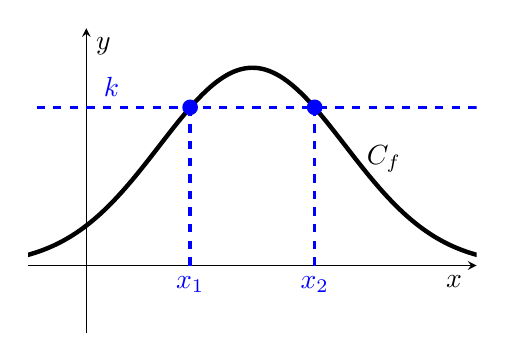
\begin{tikzpicture}[scale=1]
\begin{axis}[
axis x line=bottom,
axis y line = left,
axis lines=middle,
width=0.6*\linewidth,
height=0.45*\linewidth,
xmin=-0.5, xmax=4.5,
ymin=-1, ymax=4,
enlargelimits={abs=0.2},
xlabel={$x$},
ylabel={$y$},
%ytick distance=1,
ticks=none,
grid style=dashed,
%axis equal,
legend pos=north east,
xlabel style={at={(ticklabel* cs:0.95)},below=0.1},
]
\addplot[samples=101,smooth,ultra thick,domain=(-2:5),mark=none]{3.5*e^(-0.4*(x-2)^2)} node [pos=0.75,right] {$\mathscr C_f$};

\addplot +[mark=none,color=blue,style=dashed,very thick] coordinates {(-1,2.8) (5, 2.8)} node [pos=0.18,above right] {$k$};
\node[circle, minimum size=1pt,fill,color=blue,inner sep=2pt] at (axis cs:1.25,2.8) {};
\node[circle, minimum size=1pt,fill,color=blue,inner sep=2pt] at (axis cs:2.75,2.8) {};
\addplot +[mark=none,color=blue,style=dashed,very thick] coordinates {(1.25,0) (1.25, 2.8)} node [pos=0,below] {$x_1$};
\addplot +[mark=none,color=blue,style=dashed,very thick] coordinates {(2.75,0) (2.75, 2.8)} node [pos=0,below] {$x_2$};
%\addplot +[mark=none,color=red,style=dashed,very thick] coordinates {(-1, 0) (-1, 2)};
%\addplot +[mark=none,color=red,style=dashed,very thick] coordinates {(-1, 2) (0, 2)};
%\node[label={0:{$(0,1)$}},rectangle,fill,inner sep=2pt] at (axis cs:0,1) {};
%\node[label={[label distance=2pt]-90:{$(0,1)$}},rectangle,fill,inner sep=0pt, minimum height=0pt, minimum width=4pt] at (axis cs:1,1) {};
\end{axis}
\end{tikzpicture}}
&
\Centering{
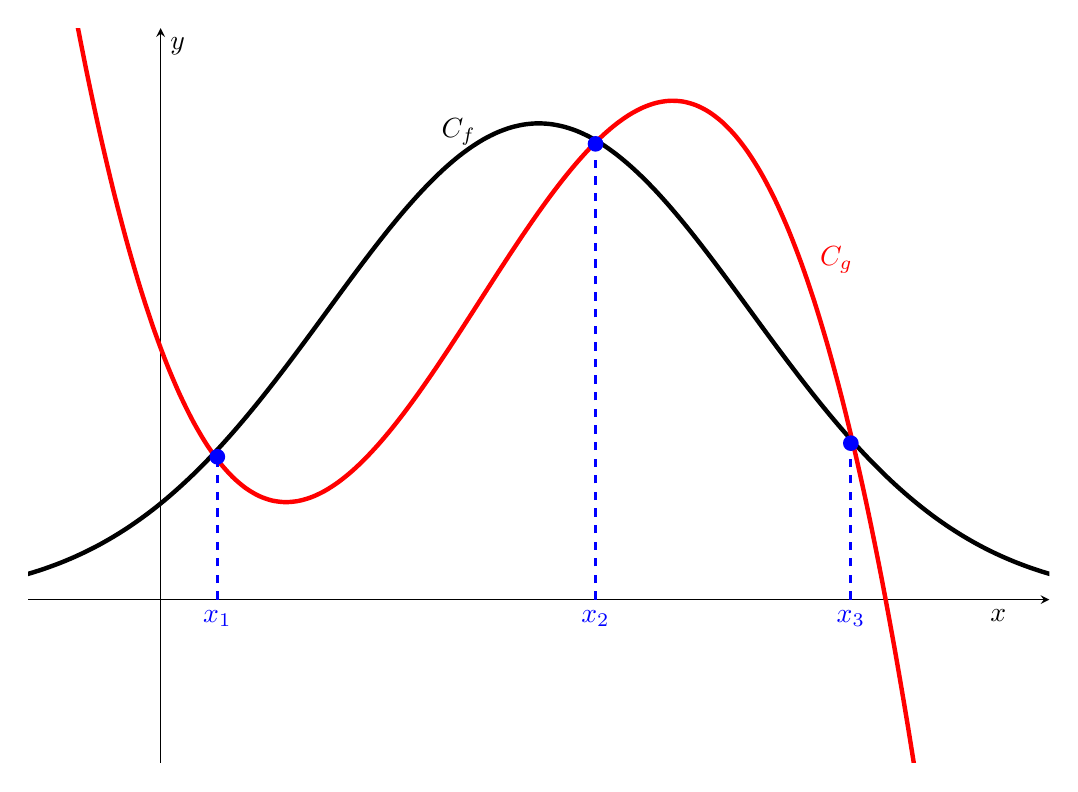
\begin{tikzpicture}[scale=1]
\begin{axis}[
axis x line=bottom,
axis y line = left,
axis lines=middle,
width=1.2*\linewidth,
height=0.9*\linewidth,
xmin=-0.5, xmax=4.5,
ymin=-1, ymax=4,
enlargelimits={abs=0.2},
xlabel={$x$},
ylabel={$y$},
ticks=none,
%ytick distance=1,
%axis equal,
yticklabel=\empty,
xticklabel=\empty,
xlabel style={at={(ticklabel* cs:0.95)},below=0.1},
]
\addplot[samples=101,smooth,ultra thick,domain=(-2:5),mark=none]{3.5*e^(-0.4*(x-2)^2)} node [pos=0.5,above] {$\mathscr C_f$};
\addplot[samples=101,smooth,ultra thick,domain=(-2:5),mark=none,color=red]{-0.69*x^3+3.49*x^2-3.72*x+1.85} node [pos=0.65,above right,color=red] {$\mathscr C_g$};

\addplot +[mark=none,color=blue,style=dashed,very thick] coordinates {(0.3,0) (0.3, 1.05)} node [pos=0,below] {$x_1$} node[pos=1,circle, minimum size=1pt,fill,inner sep=2pt] {};
\addplot +[mark=none,color=blue,style=dashed,very thick] coordinates {(2.3,0) (2.3, 3.35)} node [pos=0,below] {$x_2$} node[pos=1,circle, minimum size=1pt,fill,inner sep=2pt] {};
\addplot +[mark=none,color=blue,style=dashed,very thick] coordinates {(3.65,0) (3.65, 1.15)} node [pos=0,below] {$x_3$} node[pos=1,circle, minimum size=1pt,fill,inner sep=2pt] {};
%\addplot +[mark=none,color=red,style=dashed,very thick] coordinates {(-1, 0) (-1, 2)};
%\addplot +[mark=none,color=red,style=dashed,very thick] coordinates {(-1, 2) (0, 2)};
%\node[label={0:{$(0,1)$}},rectangle,fill,inner sep=2pt] at (axis cs:0,1) {};
%\node[label={[label distance=2pt]-90:{$(0,1)$}},rectangle,fill,inner sep=0pt, minimum height=0pt, minimum width=4pt] at (axis cs:1,1) {};
\end{axis}
\end{tikzpicture}}
\\ \hline
Résoudre l'inéquation $f(x) \geq k$ signifie trouver les nombres qui ont une image supérieure à $k$.

Cela revient donc à chercher l'abscisse des points de la courbe se situant "au dessus" de la droite d'équation $y=k$.

Ici, l'ensemble des solution de l'équation est:$$S=\left[ x_1;x_2 \right]$$ \vspace{-5mm}
&
Résoudre l'inéquation $f(x)<k$ signifie trouver les nombres qui ont une image inférieure à $k$.

Cela revient donc à chercher l'abscisse des points de la courbe se situant "en dessous" de la droite d'équation $y=k$.

Ici, l'ensemble des solution de l'équation est:$$S=\left] - \infty;x_1 \right[ \cup \left] x_2 ; + \infty \right[$$ \vspace{-5mm}
&
Résoudre l'inéquation $f(x) > g(x)$ signifie trouver les nombres dont l'image par $f$ est supérieure à l'image par $g$.

Cela revient à chercher l'abscisse des points de $\mathscr C_f$ situés "au dessus" des points de $\mathscr C_g$. \vspace{-5mm} \\ \hline
\end{tabularx}}
\end{center}

\rem{Exos Hyperbole}
\renewcommand\tabularxcolumn[1]{m{#1}}
\section{Etudes de fonctions}

\subsection{Etude des variations}

Soit $f$ définie sur un intervalle $I$.
\begin{itemize}
\item On dit que $f$ est croissante sur I si lorsque la variable augmente dans $I$, les images augmentent aussi : Pour $x,y \in I$, si $x \leq y$ alors $f(x) \leq f(y)$.:
\item On dit que $f$ est décroissante sur I si lorsque la variable augmente dans $I$, les images diminuent: Pour $x,y \in I$, si $x \leq y$ alors $f(x) \geq f(y)$.
\item On dit que $f$ est monotone sur I si elle est soit croissante, soit décroissante sur I ( son sens de variation ne change pas ).
\end{itemize}

\begin{methode}
Dresser le tableau de variations d'une fonction $f$, c'est indiquer sur quels intervalles la fonction $f$ est croissante, décroissante ou constante.

\compo[0.45]{
\begin{center}
\begin{tikzpicture}[scale=\echellepgf]
\begin{axis}[
styleglobal,
width=1*\echellepgfinv*\linewidth,
xmin=-3, xmax=6,
ymin=-1, ymax=5,
ytick distance=2,
xtick distance=2
%scale=0.7
]
\addplot[samples=101,smooth,ultra thick,domain=(0:4),mark=none] plot coordinates {(-2,2) (-1,5) (1,0) (2,-1) (4,0) (5,2)} node [pos=0.9,above left] {$\mathscr C_f$};

\end{axis}
\end{tikzpicture}
\end{center}
}
{

%:-+-+-+-+- Engendré par : http://math.et.info.free.fr/TikZ/TableauxVariations/
\begin{center}
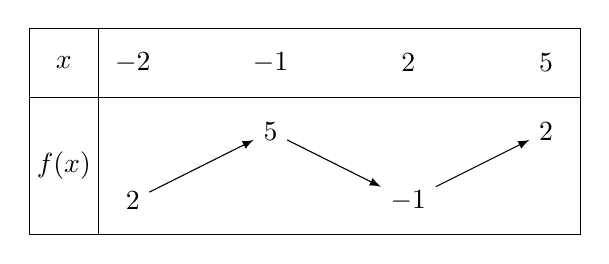
\begin{tikzpicture}[scale=0.875]
% Styles 
\tikzstyle{cadre}=[thin]
\tikzstyle{fleche}=[->,>=latex,thin]
\tikzstyle{nondefini}=[lightgray]
% Dimensions Modifiables
\def\Lrg{1}
\def\HtX{1}
\def\HtY{0.5}
% Dimensions Calculées
\def\lignex{-0.5*\HtX}
\def\lignef{-1.5*\HtX}
\def\separateur{-0.5*\Lrg}
% Largeur du tableau
\def\gauche{-1.5*\Lrg}
\def\droite{6.5*\Lrg}
% Hauteur du tableau
\def\haut{0.5*\HtX}
\def\bas{-1.5*\HtX-2*\HtY}
% Ligne de l'abscisse : x
\node at (-1*\Lrg,0) {$x$};
\node at (0*\Lrg,0) {$-2$};
\node at (2*\Lrg,0) {$-1$};
\node at (4*\Lrg,0) {$2$};
\node at (6*\Lrg,0) {$5$};
% Ligne de la fonction : f(x)
\node  at (-1*\Lrg,{-1*\HtX+(-1)*\HtY}) {$f(x)$};
\node (f1) at (0*\Lrg,{-1*\HtX+(-2)*\HtY}) {$2$};
\node (f2) at (2*\Lrg,{-1*\HtX+(0)*\HtY}) {$5$};
\node (f3) at (4*\Lrg,{-1*\HtX+(-2)*\HtY}) {$-1$};
\node (f4) at (6*\Lrg,{-1*\HtX+(0)*\HtY}) {$2$};
% Flèches
\draw[fleche] (f1) -- (f2);
\draw[fleche] (f2) -- (f3);
\draw[fleche] (f3) -- (f4);
% Encadrement
\draw[cadre] (\separateur,\haut) -- (\separateur,\bas);
\draw[cadre] (\gauche,\haut) rectangle  (\droite,\bas);
\draw[cadre] (\gauche,\lignex) -- (\droite,\lignex);
\end{tikzpicture}
\end{center}
%:-+-+-+-+- Fin

%:>>>>> code du tableau à ré-injecter
%[
%	["x", "f'(x)", "f(x)"],
%	["-2", "", "+", "2"],
%	["-1", "", "-", "5"],
%	["2", "", "+", "-1"],
%	["5", "", "?", "2"]
%]
}
\end{methode}

\subsection{Etude du signe}

\begin{methode}
Dresser le tableau de signes d'une fonction $f$, c'est indiquer sur quels intervalles la fonction est négative, positive ou nulle.

Avec la même fonction que précédemment, on obtient:
%:-+-+-+-+- Engendré par : http://math.et.info.free.fr/TikZ/TableauxVariations/
\begin{center}
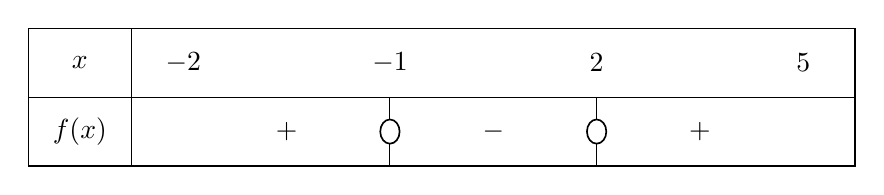
\begin{tikzpicture}[scale=0.875]
% Styles 
\tikzstyle{cadre}=[thin]
\tikzstyle{fleche}=[->,>=latex,thin]
\tikzstyle{nondefini}=[lightgray]
% Dimensions Modifiables
\def\Lrg{1.5}
\def\HtX{1}
\def\HtY{0.5}
% Dimensions Calculées
\def\lignex{-0.5*\HtX}
\def\lignef{-1.5*\HtX}
\def\separateur{-0.5*\Lrg}
% Largeur du tableau
\def\gauche{-1.5*\Lrg}
\def\droite{6.5*\Lrg}
% Hauteur du tableau
\def\haut{0.5*\HtX}
\def\bas{-2.5*\HtX-2*\HtY}
% Ligne de l'abscisse : x
\node at (-1*\Lrg,0) {$x$};
\node at (0*\Lrg,0) {$-2$};
\node at (2*\Lrg,0) {$-1$};
\node at (4*\Lrg,0) {$2$};
\node at (6*\Lrg,0) {$5$};
% Ligne de la dérivée : f'(x)
\node at (-1*\Lrg,-1*\HtX) {$f(x)$};
\node at (1*\Lrg,-1*\HtX) {$+$};
\node at (3*\Lrg,-1*\HtX) {$-$};
\node at (5*\Lrg,-1*\HtX) {$+$};
\draw[cadre] (2*\Lrg,-0.5*\HtX) -- (2*\Lrg,-1.5*\HtX) node[pos=0.5,line width=0.6pt,draw=black,circle,minimum size=7pt,fill=white,inner sep=2pt,yscale=1.25] {};
\draw[cadre] (4*\Lrg,-0.5*\HtX) -- (4*\Lrg,-1.5*\HtX) node[pos=0.5,line width=0.6pt,draw=black,circle,minimum size=7pt,fill=white,inner sep=2pt,yscale=1.25] {};
% Ligne de la fonction : f(x)
% Encadrement
\draw[cadre] (\separateur,\haut) -- (\separateur, \lignef);
\draw[cadre] (\gauche,\haut) rectangle  (\droite, \lignef);
\draw[cadre] (\gauche,\lignex) -- (\droite,\lignex);
\end{tikzpicture}
\end{center}
%:-+-+-+-+- Fin

%:>>>>> code du tableau à ré-injecter
%[
%	["x", "f(x)", ""],
%	["-2", "", "+", ""],
%	["-1", "0", "-", ""],
%	["2", "0", "+", ""],
%	["5", "", "?", ""]
%]

\end{methode}

\section{Parité d'une fonction}

\begin{defin}
Soit $f$ une fonction définie sur un intervalle $I$ centré en $0$ ( $I=[-a;a]$, $]-a;a[$ ou $\R$). On dit que f est:
\begin{itemize}
\item \textbf{paire} lorsque pour tout $x \in I, f(-x)=f(x)$.
\item \textbf{impaire} lorsque pour tout $x \in I, f(-x)=-f(x)$.
\end{itemize}
\end{defin}

\begin{exs} \
\begin{itemize}
\item La fonction $\fonction f {[-2;2]} {\R} x {x^2-1}$ est paire car pour tout $x \in [-2;2], f(-x)=(-x)^2-1=x^2-1=f(x)$.
\item La fonction $\fonction g {]3;3[} {\R} x {0.5x}$ est impaire.
\end{itemize}
\end{exs}

\begin{proprs} \
\begin{itemize}
\item $f$ est paire si et seulement si $\mathscr C_f$ est symétrique par rapport à l'axe des ordonnées.
\item $f$ est impaire si et seulement si $\mathscr C_f$ est symétrique par rapport à l'origine du repère $(0;0)$.
\end{itemize}
\end{proprs}
\begin{centrer}
\begin{tikzpicture}[scale=\echellepgf]
\begin{axis}[
styleglobal,
width=0.9*\echellepgfinv*\linewidth,
xmin=-6, xmax=6,
ymin=-1.5, ymax=3,
]
\addplot[samples=101,smooth,ultra thick,domain=(-4:4),mark=none]{0.25*x^2-1} node [pos=0.9,right] {$\mathscr C_f$};
%\addlegendentry{$f(x)=x^2-1$};
\addplot[samples=101,smooth,ultra thick,domain=(-6:6),mark=none,color=blue]{0.25*x} node [pos=0.85,below right] {$\mathscr C_g$};
%\addlegendentry{$g(x)=0.5x$};

\end{axis}
\end{tikzpicture}
\end{centrer}

\begin{rmq}
Une fonction peut être ni paire ni impaire!
\end{rmq}

\newpage

\newpage

Déroulé:

\begin{itemize}
\item \textbf{Total: 3.5 semaines ( 4-4.5 si signes/variations )}
\item Semaine 1
\begin{itemize} 
\item 1h30 - Activité intro ( coordonnées points, graphes )
\item 30m - Début du cours: I
\end{itemize}
\item Vacances - Semaine 2  
\begin{itemize}
\item 30m - Activité Emmanuel (remise en marche) - Questions 1 à 8
\item 3h - Cours II puis Exos 1 -> 8  (TD Chingatome en +)
\end{itemize}
\item Semaine 3
\begin{itemize}
\item 2h30 - Cours (in)equations + Exos Hyperbole
\item 1h30 - Parité
\end{itemize}
\end{itemize}

Compétences: 

\begin{itemize}
\item Fonctions à valeurs réelles définies sur un intervalle ou une réunion finie d'intervalles
\item Courbe représentative: $(x,f(x))$ \ldots
\item Fonction paire, impaire. Traduction géométrique
\item Capacités:
\begin{itemize}
\item Exploiter l'équation d'une courbe: appartenance, coordonnées
\item Modéliser par des fonctions [ \ldots ]
\item Résoudre des (in)équations: graphiquement, algébriquement, tableaux de signes
\item Etudier la parité dans des cas simples
\end{itemize}
\item Croissance, décroissance, monotonie, tableaux de variations
\end{itemize}
\end{document}
